\documentclass{article} % For LaTeX2e
\usepackage{nips13submit_e,times}
\usepackage{hyperref}
\usepackage{url}
\usepackage{booktabs}
\usepackage{graphicx}
\usepackage{amsfonts}
\usepackage{mathtools}
%\documentstyle[nips13submit_09,times,art10]{article} % For LaTeX 2.09

\DeclarePairedDelimiter\abs{\lvert}{\rvert}%
\DeclarePairedDelimiter\norm{\lVert}{\rVert}%

% Swap the definition of \abs* and \norm*, so that \abs
% and \norm resizes the size of the brackets, and the 
% starred version does not.
\makeatletter
\let\oldabs\abs
\def\abs{\@ifstar{\oldabs}{\oldabs*}}
%
\let\oldnorm\norm
\def\norm{\@ifstar{\oldnorm}{\oldnorm*}}
\makeatother


\title{Projet}


\author{
Olivier Gagnon \And Bernard Lebel
}

% The \author macro works with any number of authors. There are two commands
% used to separate the names and addresses of multiple authors: \And and \AND.
%
% Using \And between authors leaves it to \LaTeX{} to determine where to break
% the lines. Using \AND forces a linebreak at that point. So, if \LaTeX{}
% puts 3 of 4 authors names on the first line, and the last on the second
% line, try using \AND instead of \And before the third author name.

\newcommand{\fix}{\marginpar{FIX}}
\newcommand{\new}{\marginpar{NEW}}

\nipsfinalcopy % Uncomment for camera-ready version

\begin{document}


\maketitle

\begin{abstract}

\end{abstract}

\section{Introduction}

% Describe the problem or application that your project is concerned with.
Object recognition is a classification problem where a system attempts to identify an object in a picture using classification's algorithms. Litterature shows that a common approach to this type of problems is to rely on machine learning techniques. Those techniques however tend to require a labeled dataset (i.e. a database of items with an associated classification label) onto which the system has to be trained. As extensive datasets can be costly to acquire, unsupervised machine learning methods using non-labeled data can be used to alleviate this problem. This broadens the amount of possible inputs without requiring codification by a human.

One of the information that can prove useful is temporal coherence. Temporal coherence is a principle that states that in a video sequence, it is likely that two adjacent frames contains the same objects rather than radically different ones. Interestingly, this statement can also be considered true in other field of studies where data is of sequential nature (e.g. biological sensor inputs).

The method chosen to solve this problem is to use temporal coherence as a regularizer to exploit this information in unlabeled temporal data.\cite{?}
%Mention the method you have chosen and why it solves your problem or is a good choice for your application.
This method is a good choice for our problem, because it accounts for the likelihood that two consequent frames in a video contains the same object and that two distant frames are likely not. Leveraging this approach, it is stipulated that a neural network can be trained using standard labeled inputs, sequential non-labeled inputs and non-sequential non-labeled inputs altogether to achieve an accurate object categorization in context where inputs are non-sequential. 

\section{Description}
\subsection{COIL100 dataset}
%-Describe in detail your method / algorithm implementation. Here are some things that you could discuss :
%    – Description of the data.
%    – Description and notation for the inputs.
%    – Description and notation for the targets.

The dataset used in this project is the COIL100 dataset\cite{?}. This dataset presents the pictures of 100 objects placed on a turntable and rotated by increments of 5 degrees by picture. It contains 72 images by object, for a total of 7200 pictures. The input consists of RGB images in the Gif format and the target is an integer from 1 to 100.

\begin{figure}[h]
\label{fig:coil100}
\center
\includegraphics[scale=1]{../../images/obj67__220.png} 
\includegraphics[scale=1]{../../images/obj23__220.png} 
\includegraphics[scale=1]{../../images/obj26__220.png} 
\includegraphics[scale=1]{../../images/obj13__220.png} 
\includegraphics[scale=1]{../../images/obj29__220.png}  
\includegraphics[scale=1]{../../images/obj67__110.png} 
\includegraphics[scale=1]{../../images/obj23__110.png} 
\includegraphics[scale=1]{../../images/obj26__110.png} 
\includegraphics[scale=1]{../../images/obj13__110.png} 
\includegraphics[scale=1]{../../images/obj29__110.png}  
\caption{Examples from the coil100 dataset}
\end{figure}

\subsection{Algorithm}
%– Write a description of the general principles behind your approach. Here are some things that you could discuss :
%    – Type of learning (supervised / unsupervised, discriminative / generative).
%    – Intuition behind the training objective your algorithm optimizes.
%    – Intuition behind the architecture of the neural network.
The algorithm implemented in this project is a semi-supervised algorithm. The base algorithm used is a convolutionnal neural network (CNN) trained as a classifier on the dataset COIL-100~\cite{?}. A regularizer is then applied to ensure that the CNN does not act in a radically different manner for two consecutives unlabelled video-frame. A second regularization is also applied to ensure that two non-consecutives frame do not act in the same way.

%– Provide a detailed description of your algorithm which implements these principles. Your description should allow a person to reimplement your method from your description. Here are some things that you could discuss :
%    – Objective optimized during training. X
%    – Optimization technique used. X
%    – Description of gradients. 1/2X
%    – Architecture of the neural network. X
%    – Training procedure (one phase of training or training in several phases).
%    – Description of the use of the network to make a prediction on new data.
%    - Description of hyper-parameters.
%    – Pseudocodes of your algorithm.
\subsection{Details}
The CNN~\cite{?} architecture is presented in the figure~\ref{fig:convolutionnal-neural-net}. It consists in a chain of filters and resolution reduction steps. CNN are a good choice for visual recognition tasks because they can take the 2D topology of the data into account and because their structure limits the number of parameters to be learned. Additionally, the filter during the convolutions phases create a system that resists well to translations of a target in a picture. 
\begin{figure}[h]
\label{fig:convolutionnal-neural-net}
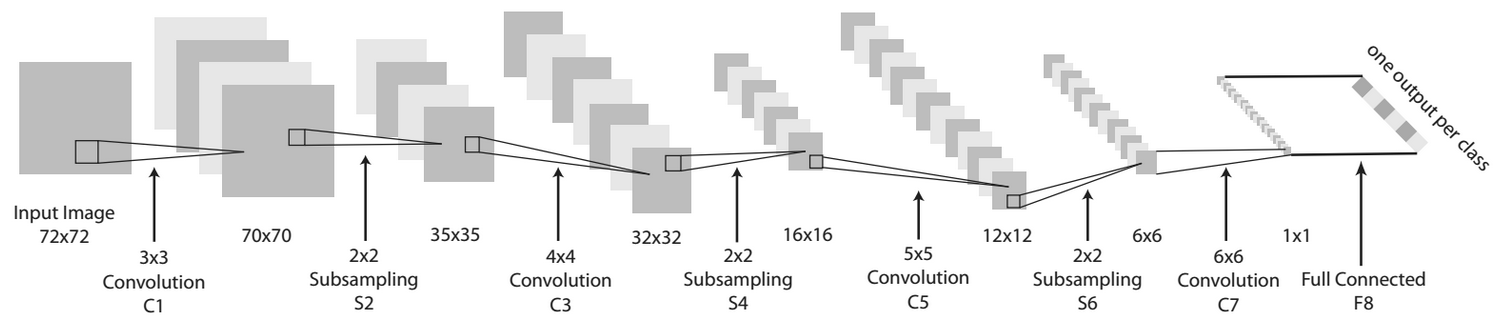
\includegraphics[width=\textwidth]{CNN.png}
\caption{A convolutionnal neural network}
\end{figure}

\subsubsection{Convolution and subsampling}

The convolution layer $C_l$ in the architecture presented in figure~\ref{fig:convolutionnal-neural-net} does a linear $K^l \times K^l$ filtering over the the image input planes $z^{l-1}_{1... N^{l-1}}$. A number of planes $z^l_{1...N^l}$ are output, where the value at position $(i, j)$ is given by:
\begin{equation}
z^l_p(i,j) = \abs{\sum_q \sum_{s=1}^{K^l} \sum_{t=1}^{K^l} w^l_{p,q,s,t}z_q^{l-1}(i-1+s, j-1+t)}
\end{equation}
%TODO Removed b^l_p + because how computations does not include it.
Where $b^l_p$ and $w^l_{p,q,s,t}$ are learned by backpropagation. The absolute value is taken to create an invariance to the direction of the edges in the edge detection filters.

The subsampling is done by taking the maximum value over non-overlapping windows.

A $\tanh()$ function is applied after the maxpooling layer to induce a non-linearity.

Finally, a last layer is a fully-connected layer which outputs one value per class. A "softmax" layer is then added to compute a probability:
\begin{equation}
\tilde{P_p} = \frac{\exp (z_p^{l-1})}{\sum_q \exp (z_q^{l-1})}
\end{equation}

\subsection{Optimization}

Three cost functions are optimized during training. In each case, stochastic gradients descent is used~\cite{?} .

The first cost function is the negative log-likelihood $L(\mathbf{\theta}) = \sum_{n=1}^N L(\mathbf{\theta},\mathbf{x}_n, y_n)$.

The gradient descent update is as follow:
\begin{equation}
\theta \leftarrow \theta - \lambda \frac{\partial L(\theta, \mathbf{x}
, y)}{\partial \theta}
\end{equation}
where $\lambda$ is a learning rate.

The second and third lost functions are presented in \cite{?}.

Considering two images $\mathbf{x_1}$ and $\mathbf{x_2}$ and their respective representation in the $l^{th}$ layer $z_\theta^l(\mathbf{x_1})$ and $z_\theta^l(\mathbf{x_2})$, we enforce $z_\theta^l(\mathbf{x_1})$ and $z_\theta^l(\mathbf{x_2})$ to be close when the two images are consecutive frames in a video.

\begin{equation}
L_{coh1}(\theta, \mathbf{x_1}, \mathbf{x_2}) = \norm{z_\theta^l(\mathbf{x_1}) - z_\theta^l(\mathbf{x_2})}_1
\end{equation}

Finally, the third cost function is the opposite of the last one. That is, considering two images $\mathbf{x_1}$ and $\mathbf{x_2}$ and their respective representation in the $l^{th}$ layer $z_\theta^l(\mathbf{x_1})$ and $z_\theta^l(\mathbf{x_2})$, we enforce $z_\theta^l(\mathbf{x_1})$ and $z_\theta^l(\mathbf{x_2})$ to be different when the two images are randomly picked in the video under the assumption that they have an higher risk of representing different objects.

\begin{equation}
L_{coh2}(\theta, \mathbf{x_1}, \mathbf{x_2}) = \max \left(0, \delta - \norm{z_\theta^l(\mathbf{x_1}) - z_\theta^l(\mathbf{x_2})}_1\right)
\end{equation}
where $\delta$ is a margin that could be chosen as an hyperparameter. However, just as in~\cite{}, the value of $\delta$ is fixed to 1.

\section{Results}
%TODO – Describe your experimental protocol (proportions used to divide the data into training, validation and test sets, data preprocessing, etc.).
%TODO – Describe your procedure for selecting hyper-parameters.
%TODO – Present and analyze the results for different hyper-parameters on the validation and training sets.
%TODO – Present any results that validate the correctness of your implementation.
%TODO – Present the results of your algorithm on the test set and make a comparison with an alternative, simple baseline.
\end{document}
